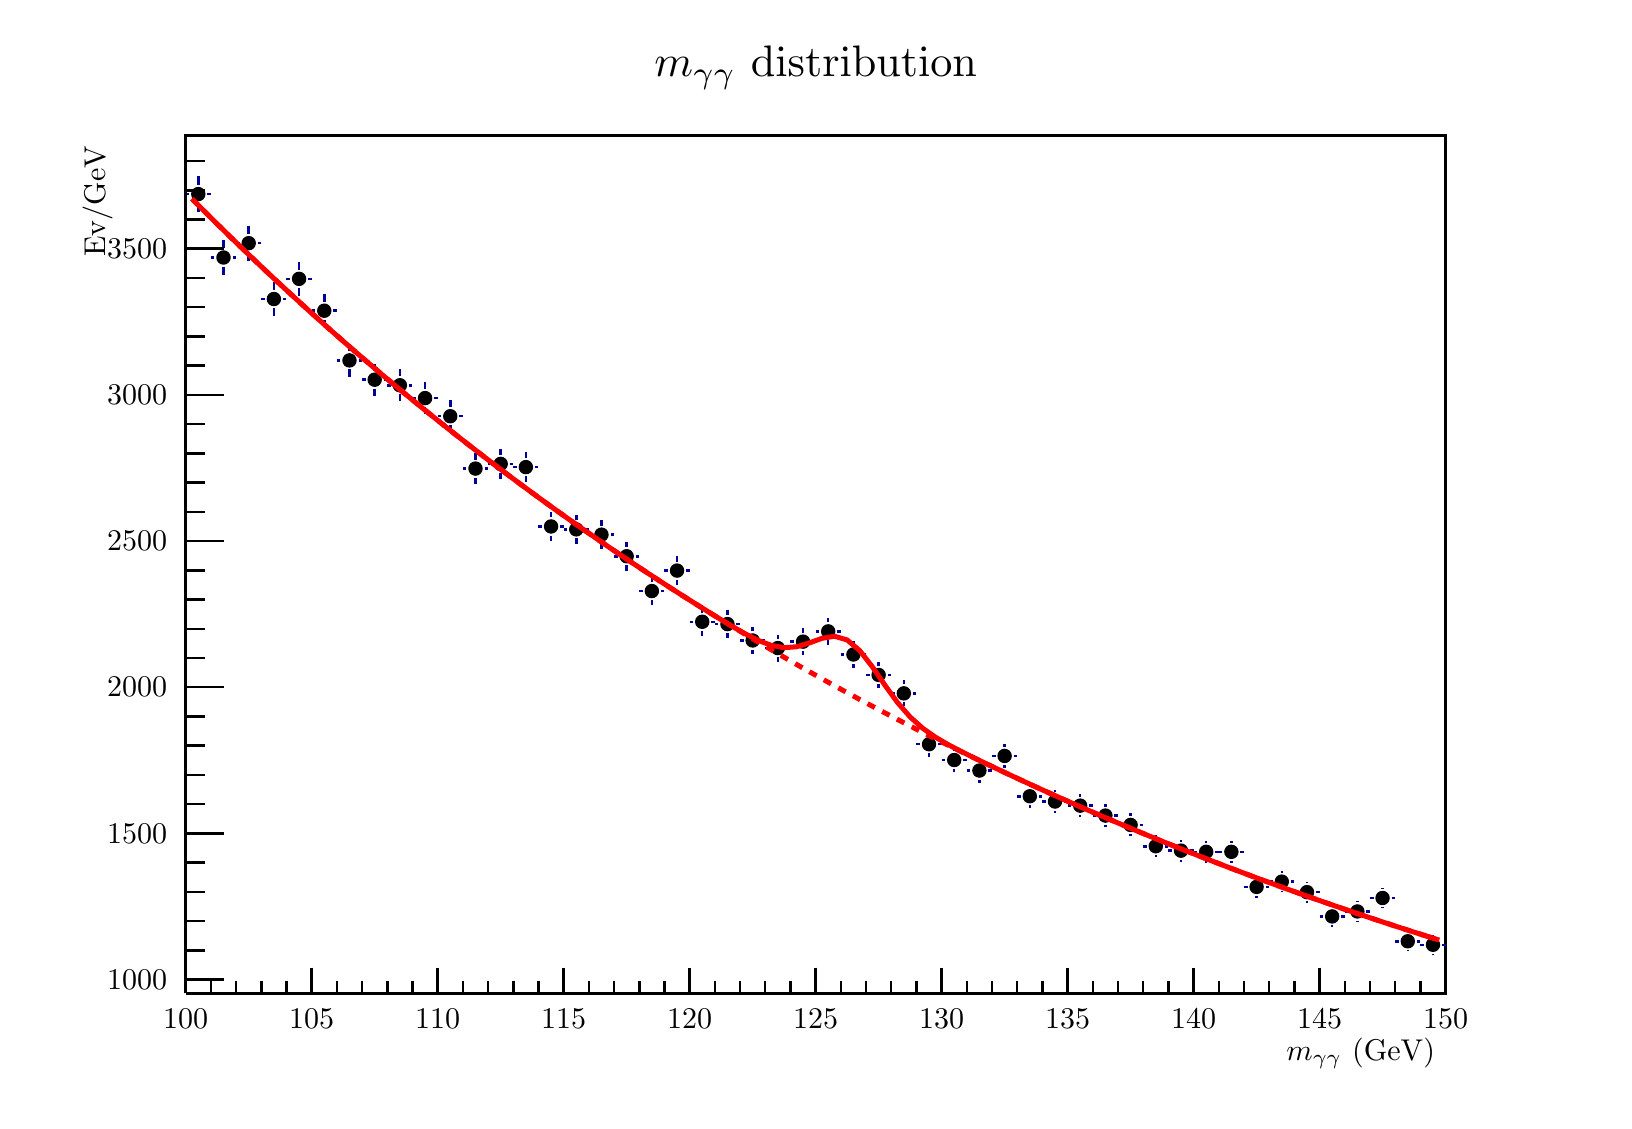
\begin{tikzpicture}
\pgfdeclareplotmark{cross} {
\pgfpathmoveto{\pgfpoint{-0.3\pgfplotmarksize}{\pgfplotmarksize}}
\pgfpathlineto{\pgfpoint{+0.3\pgfplotmarksize}{\pgfplotmarksize}}
\pgfpathlineto{\pgfpoint{+0.3\pgfplotmarksize}{0.3\pgfplotmarksize}}
\pgfpathlineto{\pgfpoint{+1\pgfplotmarksize}{0.3\pgfplotmarksize}}
\pgfpathlineto{\pgfpoint{+1\pgfplotmarksize}{-0.3\pgfplotmarksize}}
\pgfpathlineto{\pgfpoint{+0.3\pgfplotmarksize}{-0.3\pgfplotmarksize}}
\pgfpathlineto{\pgfpoint{+0.3\pgfplotmarksize}{-1.\pgfplotmarksize}}
\pgfpathlineto{\pgfpoint{-0.3\pgfplotmarksize}{-1.\pgfplotmarksize}}
\pgfpathlineto{\pgfpoint{-0.3\pgfplotmarksize}{-0.3\pgfplotmarksize}}
\pgfpathlineto{\pgfpoint{-1.\pgfplotmarksize}{-0.3\pgfplotmarksize}}
\pgfpathlineto{\pgfpoint{-1.\pgfplotmarksize}{0.3\pgfplotmarksize}}
\pgfpathlineto{\pgfpoint{-0.3\pgfplotmarksize}{0.3\pgfplotmarksize}}
\pgfpathclose
\pgfusepathqstroke
}
\pgfdeclareplotmark{cross*} {
\pgfpathmoveto{\pgfpoint{-0.3\pgfplotmarksize}{\pgfplotmarksize}}
\pgfpathlineto{\pgfpoint{+0.3\pgfplotmarksize}{\pgfplotmarksize}}
\pgfpathlineto{\pgfpoint{+0.3\pgfplotmarksize}{0.3\pgfplotmarksize}}
\pgfpathlineto{\pgfpoint{+1\pgfplotmarksize}{0.3\pgfplotmarksize}}
\pgfpathlineto{\pgfpoint{+1\pgfplotmarksize}{-0.3\pgfplotmarksize}}
\pgfpathlineto{\pgfpoint{+0.3\pgfplotmarksize}{-0.3\pgfplotmarksize}}
\pgfpathlineto{\pgfpoint{+0.3\pgfplotmarksize}{-1.\pgfplotmarksize}}
\pgfpathlineto{\pgfpoint{-0.3\pgfplotmarksize}{-1.\pgfplotmarksize}}
\pgfpathlineto{\pgfpoint{-0.3\pgfplotmarksize}{-0.3\pgfplotmarksize}}
\pgfpathlineto{\pgfpoint{-1.\pgfplotmarksize}{-0.3\pgfplotmarksize}}
\pgfpathlineto{\pgfpoint{-1.\pgfplotmarksize}{0.3\pgfplotmarksize}}
\pgfpathlineto{\pgfpoint{-0.3\pgfplotmarksize}{0.3\pgfplotmarksize}}
\pgfpathclose
\pgfusepathqfillstroke
}
\pgfdeclareplotmark{newstar} {
\pgfpathmoveto{\pgfqpoint{0pt}{\pgfplotmarksize}}
\pgfpathlineto{\pgfqpointpolar{44}{0.5\pgfplotmarksize}}
\pgfpathlineto{\pgfqpointpolar{18}{\pgfplotmarksize}}
\pgfpathlineto{\pgfqpointpolar{-20}{0.5\pgfplotmarksize}}
\pgfpathlineto{\pgfqpointpolar{-54}{\pgfplotmarksize}}
\pgfpathlineto{\pgfqpointpolar{-90}{0.5\pgfplotmarksize}}
\pgfpathlineto{\pgfqpointpolar{234}{\pgfplotmarksize}}
\pgfpathlineto{\pgfqpointpolar{198}{0.5\pgfplotmarksize}}
\pgfpathlineto{\pgfqpointpolar{162}{\pgfplotmarksize}}
\pgfpathlineto{\pgfqpointpolar{134}{0.5\pgfplotmarksize}}
\pgfpathclose
\pgfusepathqstroke
}
\pgfdeclareplotmark{newstar*} {
\pgfpathmoveto{\pgfqpoint{0pt}{\pgfplotmarksize}}
\pgfpathlineto{\pgfqpointpolar{44}{0.5\pgfplotmarksize}}
\pgfpathlineto{\pgfqpointpolar{18}{\pgfplotmarksize}}
\pgfpathlineto{\pgfqpointpolar{-20}{0.5\pgfplotmarksize}}
\pgfpathlineto{\pgfqpointpolar{-54}{\pgfplotmarksize}}
\pgfpathlineto{\pgfqpointpolar{-90}{0.5\pgfplotmarksize}}
\pgfpathlineto{\pgfqpointpolar{234}{\pgfplotmarksize}}
\pgfpathlineto{\pgfqpointpolar{198}{0.5\pgfplotmarksize}}
\pgfpathlineto{\pgfqpointpolar{162}{\pgfplotmarksize}}
\pgfpathlineto{\pgfqpointpolar{134}{0.5\pgfplotmarksize}}
\pgfpathclose
\pgfusepathqfillstroke
}
\definecolor{c}{rgb}{1,1,1};
\draw [color=c, fill=c] (0,0) rectangle (20,13.6207);
\draw [color=c, fill=c] (2,1.36207) rectangle (18,12.2586);
\definecolor{c}{rgb}{0,0,0};
\draw [c,line width=0.9] (2,1.36207) -- (2,12.2586) -- (18,12.2586) -- (18,1.36207) -- (2,1.36207);
\definecolor{c}{rgb}{1,1,1};
\draw [color=c, fill=c] (2,1.36207) rectangle (18,12.2586);
\definecolor{c}{rgb}{0,0,0};
\draw [c,line width=0.9] (2,1.36207) -- (2,12.2586) -- (18,12.2586) -- (18,1.36207) -- (2,1.36207);
\definecolor{c}{rgb}{0,0,0.6};
\draw [c,line width=0.9] (2.16,11.2889) -- (2.16,11.3994);
\draw [c,line width=0.9] (2.16,11.6292) -- (2.16,11.7397);
\draw [c,line width=0.9] (2,11.5143) -- (2.04506,11.5143);
\draw [c,line width=0.9] (2.27494,11.5143) -- (2.32,11.5143);
\definecolor{c}{rgb}{0,0,0};
\foreach \P in {(2.16,11.5143)}{\draw[mark options={color=c,fill=c},mark size=2.402402pt,mark=*] plot coordinates {\P};}
\definecolor{c}{rgb}{0,0,0.6};
\draw [c,line width=0.9] (2.48,10.49) -- (2.48,10.5937);
\draw [c,line width=0.9] (2.48,10.8236) -- (2.48,10.9274);
\draw [c,line width=0.9] (2.32,10.7087) -- (2.36506,10.7087);
\draw [c,line width=0.9] (2.59494,10.7087) -- (2.64,10.7087);
\definecolor{c}{rgb}{0,0,0};
\foreach \P in {(2.48,10.7087)}{\draw[mark options={color=c,fill=c},mark size=2.402402pt,mark=*] plot coordinates {\P};}
\definecolor{c}{rgb}{0,0,0.6};
\draw [c,line width=0.9] (2.8,10.6704) -- (2.8,10.7757);
\draw [c,line width=0.9] (2.8,11.0055) -- (2.8,11.1108);
\draw [c,line width=0.9] (2.64,10.8906) -- (2.68506,10.8906);
\draw [c,line width=0.9] (2.91494,10.8906) -- (2.96,10.8906);
\definecolor{c}{rgb}{0,0,0};
\foreach \P in {(2.8,10.8906)}{\draw[mark options={color=c,fill=c},mark size=2.402402pt,mark=*] plot coordinates {\P};}
\definecolor{c}{rgb}{0,0,0.6};
\draw [c,line width=0.9] (3.12,9.96732) -- (3.12,10.0666);
\draw [c,line width=0.9] (3.12,10.2964) -- (3.12,10.3957);
\draw [c,line width=0.9] (2.96,10.1815) -- (3.00506,10.1815);
\draw [c,line width=0.9] (3.23494,10.1815) -- (3.28,10.1815);
\definecolor{c}{rgb}{0,0,0};
\foreach \P in {(3.12,10.1815)}{\draw[mark options={color=c,fill=c},mark size=2.402402pt,mark=*] plot coordinates {\P};}
\definecolor{c}{rgb}{0,0,0.6};
\draw [c,line width=0.9] (3.44,10.2213) -- (3.44,10.3227);
\draw [c,line width=0.9] (3.44,10.5526) -- (3.44,10.654);
\draw [c,line width=0.9] (3.28,10.4377) -- (3.32506,10.4377);
\draw [c,line width=0.9] (3.55494,10.4377) -- (3.6,10.4377);
\definecolor{c}{rgb}{0,0,0};
\foreach \P in {(3.44,10.4377)}{\draw[mark options={color=c,fill=c},mark size=2.402402pt,mark=*] plot coordinates {\P};}
\definecolor{c}{rgb}{0,0,0.6};
\draw [c,line width=0.9] (3.76,9.82011) -- (3.76,9.91805);
\draw [c,line width=0.9] (3.76,10.1479) -- (3.76,10.2459);
\draw [c,line width=0.9] (3.6,10.033) -- (3.64506,10.033);
\draw [c,line width=0.9] (3.87494,10.033) -- (3.92,10.033);
\definecolor{c}{rgb}{0,0,0};
\foreach \P in {(3.76,10.033)}{\draw[mark options={color=c,fill=c},mark size=2.402402pt,mark=*] plot coordinates {\P};}
\definecolor{c}{rgb}{0,0,0.6};
\draw [c,line width=0.9] (4.08,9.19455) -- (4.08,9.28691);
\draw [c,line width=0.9] (4.08,9.5168) -- (4.08,9.60916);
\draw [c,line width=0.9] (3.92,9.40186) -- (3.96506,9.40186);
\draw [c,line width=0.9] (4.19494,9.40186) -- (4.24,9.40186);
\definecolor{c}{rgb}{0,0,0};
\foreach \P in {(4.08,9.40186)}{\draw[mark options={color=c,fill=c},mark size=2.402402pt,mark=*] plot coordinates {\P};}
\definecolor{c}{rgb}{0,0,0.6};
\draw [c,line width=0.9] (4.4,8.95173) -- (4.4,9.04188);
\draw [c,line width=0.9] (4.4,9.27177) -- (4.4,9.36193);
\draw [c,line width=0.9] (4.24,9.15683) -- (4.28506,9.15683);
\draw [c,line width=0.9] (4.51494,9.15683) -- (4.56,9.15683);
\definecolor{c}{rgb}{0,0,0};
\foreach \P in {(4.4,9.15683)}{\draw[mark options={color=c,fill=c},mark size=2.402402pt,mark=*] plot coordinates {\P};}
\definecolor{c}{rgb}{0,0,0.6};
\draw [c,line width=0.9] (4.72,8.88183) -- (4.72,8.97135);
\draw [c,line width=0.9] (4.72,9.20123) -- (4.72,9.29075);
\draw [c,line width=0.9] (4.56,9.08629) -- (4.60506,9.08629);
\draw [c,line width=0.9] (4.83494,9.08629) -- (4.88,9.08629);
\definecolor{c}{rgb}{0,0,0};
\foreach \P in {(4.72,9.08629)}{\draw[mark options={color=c,fill=c},mark size=2.402402pt,mark=*] plot coordinates {\P};}
\definecolor{c}{rgb}{0,0,0.6};
\draw [c,line width=0.9] (5.04,8.71996) -- (5.04,8.80799);
\draw [c,line width=0.9] (5.04,9.03788) -- (5.04,9.12591);
\draw [c,line width=0.9] (4.88,8.92294) -- (4.92506,8.92294);
\draw [c,line width=0.9] (5.15494,8.92294) -- (5.2,8.92294);
\definecolor{c}{rgb}{0,0,0};
\foreach \P in {(5.04,8.92294)}{\draw[mark options={color=c,fill=c},mark size=2.402402pt,mark=*] plot coordinates {\P};}
\definecolor{c}{rgb}{0,0,0.6};
\draw [c,line width=0.9] (5.36,8.4919) -- (5.36,8.57781);
\draw [c,line width=0.9] (5.36,8.8077) -- (5.36,8.89361);
\draw [c,line width=0.9] (5.2,8.69276) -- (5.24506,8.69276);
\draw [c,line width=0.9] (5.47494,8.69276) -- (5.52,8.69276);
\definecolor{c}{rgb}{0,0,0};
\foreach \P in {(5.36,8.69276)}{\draw[mark options={color=c,fill=c},mark size=2.402402pt,mark=*] plot coordinates {\P};}
\definecolor{c}{rgb}{0,0,0.6};
\draw [c,line width=0.9] (5.68,7.83359) -- (5.68,7.91326);
\draw [c,line width=0.9] (5.68,8.14315) -- (5.68,8.22282);
\draw [c,line width=0.9] (5.52,8.02821) -- (5.56506,8.02821);
\draw [c,line width=0.9] (5.79494,8.02821) -- (5.84,8.02821);
\definecolor{c}{rgb}{0,0,0};
\foreach \P in {(5.68,8.02821)}{\draw[mark options={color=c,fill=c},mark size=2.402402pt,mark=*] plot coordinates {\P};}
\definecolor{c}{rgb}{0,0,0.6};
\draw [c,line width=0.9] (6,7.89242) -- (6,7.97267);
\draw [c,line width=0.9] (6,8.20255) -- (6,8.28279);
\draw [c,line width=0.9] (5.84,8.08761) -- (5.88506,8.08761);
\draw [c,line width=0.9] (6.11494,8.08761) -- (6.16,8.08761);
\definecolor{c}{rgb}{0,0,0};
\foreach \P in {(6,8.08761)}{\draw[mark options={color=c,fill=c},mark size=2.402402pt,mark=*] plot coordinates {\P};}
\definecolor{c}{rgb}{0,0,0.6};
\draw [c,line width=0.9] (6.32,7.85197) -- (6.32,7.93183);
\draw [c,line width=0.9] (6.32,8.16171) -- (6.32,8.24156);
\draw [c,line width=0.9] (6.16,8.04677) -- (6.20506,8.04677);
\draw [c,line width=0.9] (6.43494,8.04677) -- (6.48,8.04677);
\definecolor{c}{rgb}{0,0,0};
\foreach \P in {(6.32,8.04677)}{\draw[mark options={color=c,fill=c},mark size=2.402402pt,mark=*] plot coordinates {\P};}
\definecolor{c}{rgb}{0,0,0.6};
\draw [c,line width=0.9] (6.64,7.10564) -- (6.64,7.17818);
\draw [c,line width=0.9] (6.64,7.40806) -- (6.64,7.48059);
\draw [c,line width=0.9] (6.48,7.29312) -- (6.52506,7.29312);
\draw [c,line width=0.9] (6.75494,7.29312) -- (6.8,7.29312);
\definecolor{c}{rgb}{0,0,0};
\foreach \P in {(6.64,7.29312)}{\draw[mark options={color=c,fill=c},mark size=2.402402pt,mark=*] plot coordinates {\P};}
\definecolor{c}{rgb}{0,0,0.6};
\draw [c,line width=0.9] (6.96,7.06889) -- (6.96,7.14105);
\draw [c,line width=0.9] (6.96,7.37093) -- (6.96,7.4431);
\draw [c,line width=0.9] (6.8,7.25599) -- (6.84506,7.25599);
\draw [c,line width=0.9] (7.07494,7.25599) -- (7.12,7.25599);
\definecolor{c}{rgb}{0,0,0};
\foreach \P in {(6.96,7.25599)}{\draw[mark options={color=c,fill=c},mark size=2.402402pt,mark=*] plot coordinates {\P};}
\definecolor{c}{rgb}{0,0,0.6};
\draw [c,line width=0.9] (7.28,7.00272) -- (7.28,7.07422);
\draw [c,line width=0.9] (7.28,7.30411) -- (7.28,7.37561);
\draw [c,line width=0.9] (7.12,7.18917) -- (7.16506,7.18917);
\draw [c,line width=0.9] (7.39494,7.18917) -- (7.44,7.18917);
\definecolor{c}{rgb}{0,0,0};
\foreach \P in {(7.28,7.18917)}{\draw[mark options={color=c,fill=c},mark size=2.402402pt,mark=*] plot coordinates {\P};}
\definecolor{c}{rgb}{0,0,0.6};
\draw [c,line width=0.9] (7.6,6.73075) -- (7.6,6.79949);
\draw [c,line width=0.9] (7.6,7.02938) -- (7.6,7.09812);
\draw [c,line width=0.9] (7.44,6.91444) -- (7.48506,6.91444);
\draw [c,line width=0.9] (7.71494,6.91444) -- (7.76,6.91444);
\definecolor{c}{rgb}{0,0,0};
\foreach \P in {(7.6,6.91444)}{\draw[mark options={color=c,fill=c},mark size=2.402402pt,mark=*] plot coordinates {\P};}
\definecolor{c}{rgb}{0,0,0.6};
\draw [c,line width=0.9] (7.92,6.29347) -- (7.92,6.3577);
\draw [c,line width=0.9] (7.92,6.58758) -- (7.92,6.65181);
\draw [c,line width=0.9] (7.76,6.47264) -- (7.80506,6.47264);
\draw [c,line width=0.9] (8.03494,6.47264) -- (8.08,6.47264);
\definecolor{c}{rgb}{0,0,0};
\foreach \P in {(7.92,6.47264)}{\draw[mark options={color=c,fill=c},mark size=2.402402pt,mark=*] plot coordinates {\P};}
\definecolor{c}{rgb}{0,0,0.6};
\draw [c,line width=0.9] (8.24,6.55068) -- (8.24,6.61758);
\draw [c,line width=0.9] (8.24,6.84746) -- (8.24,6.91436);
\draw [c,line width=0.9] (8.08,6.73252) -- (8.12506,6.73252);
\draw [c,line width=0.9] (8.35494,6.73252) -- (8.4,6.73252);
\definecolor{c}{rgb}{0,0,0};
\foreach \P in {(8.24,6.73252)}{\draw[mark options={color=c,fill=c},mark size=2.402402pt,mark=*] plot coordinates {\P};}
\definecolor{c}{rgb}{0,0,0.6};
\draw [c,line width=0.9] (8.56,5.90774) -- (8.56,5.96788);
\draw [c,line width=0.9] (8.56,6.19776) -- (8.56,6.2579);
\draw [c,line width=0.9] (8.4,6.08282) -- (8.44506,6.08282);
\draw [c,line width=0.9] (8.67494,6.08282) -- (8.72,6.08282);
\definecolor{c}{rgb}{0,0,0};
\foreach \P in {(8.56,6.08282)}{\draw[mark options={color=c,fill=c},mark size=2.402402pt,mark=*] plot coordinates {\P};}
\definecolor{c}{rgb}{0,0,0.6};
\draw [c,line width=0.9] (8.88,5.87835) -- (8.88,5.93818);
\draw [c,line width=0.9] (8.88,6.16806) -- (8.88,6.22789);
\draw [c,line width=0.9] (8.72,6.05312) -- (8.76506,6.05312);
\draw [c,line width=0.9] (8.99494,6.05312) -- (9.04,6.05312);
\definecolor{c}{rgb}{0,0,0};
\foreach \P in {(8.88,6.05312)}{\draw[mark options={color=c,fill=c},mark size=2.402402pt,mark=*] plot coordinates {\P};}
\definecolor{c}{rgb}{0,0,0.6};
\draw [c,line width=0.9] (9.2,5.67267) -- (9.2,5.73027);
\draw [c,line width=0.9] (9.2,5.96016) -- (9.2,6.01776);
\draw [c,line width=0.9] (9.04,5.84522) -- (9.08506,5.84522);
\draw [c,line width=0.9] (9.31494,5.84522) -- (9.36,5.84522);
\definecolor{c}{rgb}{0,0,0};
\foreach \P in {(9.2,5.84522)}{\draw[mark options={color=c,fill=c},mark size=2.402402pt,mark=*] plot coordinates {\P};}
\definecolor{c}{rgb}{0,0,0.6};
\draw [c,line width=0.9] (9.52,5.57719) -- (9.52,5.63375);
\draw [c,line width=0.9] (9.52,5.86363) -- (9.52,5.92019);
\draw [c,line width=0.9] (9.36,5.74869) -- (9.40506,5.74869);
\draw [c,line width=0.9] (9.63494,5.74869) -- (9.68,5.74869);
\definecolor{c}{rgb}{0,0,0};
\foreach \P in {(9.52,5.74869)}{\draw[mark options={color=c,fill=c},mark size=2.402402pt,mark=*] plot coordinates {\P};}
\definecolor{c}{rgb}{0,0,0.6};
\draw [c,line width=0.9] (9.84,5.65798) -- (9.84,5.71542);
\draw [c,line width=0.9] (9.84,5.94531) -- (9.84,6.00275);
\draw [c,line width=0.9] (9.68,5.83037) -- (9.72506,5.83037);
\draw [c,line width=0.9] (9.95494,5.83037) -- (10,5.83037);
\definecolor{c}{rgb}{0,0,0};
\foreach \P in {(9.84,5.83037)}{\draw[mark options={color=c,fill=c},mark size=2.402402pt,mark=*] plot coordinates {\P};}
\definecolor{c}{rgb}{0,0,0.6};
\draw [c,line width=0.9] (10.16,5.78653) -- (10.16,5.84536);
\draw [c,line width=0.9] (10.16,6.07525) -- (10.16,6.13409);
\draw [c,line width=0.9] (10,5.96031) -- (10.0451,5.96031);
\draw [c,line width=0.9] (10.2749,5.96031) -- (10.32,5.96031);
\definecolor{c}{rgb}{0,0,0};
\foreach \P in {(10.16,5.96031)}{\draw[mark options={color=c,fill=c},mark size=2.402402pt,mark=*] plot coordinates {\P};}
\definecolor{c}{rgb}{0,0,0.6};
\draw [c,line width=0.9] (10.48,5.4964) -- (10.48,5.55207);
\draw [c,line width=0.9] (10.48,5.78196) -- (10.48,5.83763);
\draw [c,line width=0.9] (10.32,5.66701) -- (10.3651,5.66701);
\draw [c,line width=0.9] (10.5949,5.66701) -- (10.64,5.66701);
\definecolor{c}{rgb}{0,0,0};
\foreach \P in {(10.48,5.66701)}{\draw[mark options={color=c,fill=c},mark size=2.402402pt,mark=*] plot coordinates {\P};}
\definecolor{c}{rgb}{0,0,0.6};
\draw [c,line width=0.9] (10.8,5.23937) -- (10.8,5.29219);
\draw [c,line width=0.9] (10.8,5.52208) -- (10.8,5.5749);
\draw [c,line width=0.9] (10.64,5.40713) -- (10.6851,5.40713);
\draw [c,line width=0.9] (10.9149,5.40713) -- (10.96,5.40713);
\definecolor{c}{rgb}{0,0,0};
\foreach \P in {(10.8,5.40713)}{\draw[mark options={color=c,fill=c},mark size=2.402402pt,mark=*] plot coordinates {\P};}
\definecolor{c}{rgb}{0,0,0.6};
\draw [c,line width=0.9] (11.12,5.00809) -- (11.12,5.0583);
\draw [c,line width=0.9] (11.12,5.28819) -- (11.12,5.3384);
\draw [c,line width=0.9] (10.96,5.17324) -- (11.0051,5.17324);
\draw [c,line width=0.9] (11.2349,5.17324) -- (11.28,5.17324);
\definecolor{c}{rgb}{0,0,0};
\foreach \P in {(11.12,5.17324)}{\draw[mark options={color=c,fill=c},mark size=2.402402pt,mark=*] plot coordinates {\P};}
\definecolor{c}{rgb}{0,0,0.6};
\draw [c,line width=0.9] (11.44,4.36953) -- (11.44,4.41231);
\draw [c,line width=0.9] (11.44,4.6422) -- (11.44,4.68499);
\draw [c,line width=0.9] (11.28,4.52726) -- (11.3251,4.52726);
\draw [c,line width=0.9] (11.5549,4.52726) -- (11.6,4.52726);
\definecolor{c}{rgb}{0,0,0};
\foreach \P in {(11.44,4.52726)}{\draw[mark options={color=c,fill=c},mark size=2.402402pt,mark=*] plot coordinates {\P};}
\definecolor{c}{rgb}{0,0,0.6};
\draw [c,line width=0.9] (11.76,4.17142) -- (11.76,4.21183);
\draw [c,line width=0.9] (11.76,4.44172) -- (11.76,4.48213);
\draw [c,line width=0.9] (11.6,4.32678) -- (11.6451,4.32678);
\draw [c,line width=0.9] (11.8749,4.32678) -- (11.92,4.32678);
\definecolor{c}{rgb}{0,0,0};
\foreach \P in {(11.76,4.32678)}{\draw[mark options={color=c,fill=c},mark size=2.402402pt,mark=*] plot coordinates {\P};}
\definecolor{c}{rgb}{0,0,0.6};
\draw [c,line width=0.9] (12.08,4.03938) -- (12.08,4.07818);
\draw [c,line width=0.9] (12.08,4.30807) -- (12.08,4.34687);
\draw [c,line width=0.9] (11.92,4.19312) -- (11.9651,4.19312);
\draw [c,line width=0.9] (12.1949,4.19312) -- (12.24,4.19312);
\definecolor{c}{rgb}{0,0,0};
\foreach \P in {(12.08,4.19312)}{\draw[mark options={color=c,fill=c},mark size=2.402402pt,mark=*] plot coordinates {\P};}
\definecolor{c}{rgb}{0,0,0.6};
\draw [c,line width=0.9] (12.4,4.22278) -- (12.4,4.26381);
\draw [c,line width=0.9] (12.4,4.4937) -- (12.4,4.53473);
\draw [c,line width=0.9] (12.24,4.37875) -- (12.2851,4.37875);
\draw [c,line width=0.9] (12.5149,4.37875) -- (12.56,4.37875);
\definecolor{c}{rgb}{0,0,0};
\foreach \P in {(12.4,4.37875)}{\draw[mark options={color=c,fill=c},mark size=2.402402pt,mark=*] plot coordinates {\P};}
\definecolor{c}{rgb}{0,0,0.6};
\draw [c,line width=0.9] (12.72,3.71667) -- (12.72,3.75148);
\draw [c,line width=0.9] (12.72,3.98136) -- (12.72,4.01617);
\draw [c,line width=0.9] (12.56,3.86642) -- (12.6051,3.86642);
\draw [c,line width=0.9] (12.8349,3.86642) -- (12.88,3.86642);
\definecolor{c}{rgb}{0,0,0};
\foreach \P in {(12.72,3.86642)}{\draw[mark options={color=c,fill=c},mark size=2.402402pt,mark=*] plot coordinates {\P};}
\definecolor{c}{rgb}{0,0,0.6};
\draw [c,line width=0.9] (13.04,3.65067) -- (13.04,3.68465);
\draw [c,line width=0.9] (13.04,3.91454) -- (13.04,3.94851);
\draw [c,line width=0.9] (12.88,3.79959) -- (12.9251,3.79959);
\draw [c,line width=0.9] (13.1549,3.79959) -- (13.2,3.79959);
\definecolor{c}{rgb}{0,0,0};
\foreach \P in {(13.04,3.79959)}{\draw[mark options={color=c,fill=c},mark size=2.402402pt,mark=*] plot coordinates {\P};}
\definecolor{c}{rgb}{0,0,0.6};
\draw [c,line width=0.9] (13.36,3.59935) -- (13.36,3.63267);
\draw [c,line width=0.9] (13.36,3.86256) -- (13.36,3.89589);
\draw [c,line width=0.9] (13.2,3.74762) -- (13.2451,3.74762);
\draw [c,line width=0.9] (13.4749,3.74762) -- (13.52,3.74762);
\definecolor{c}{rgb}{0,0,0};
\foreach \P in {(13.36,3.74762)}{\draw[mark options={color=c,fill=c},mark size=2.402402pt,mark=*] plot coordinates {\P};}
\definecolor{c}{rgb}{0,0,0.6};
\draw [c,line width=0.9] (13.68,3.47471) -- (13.68,3.50645);
\draw [c,line width=0.9] (13.68,3.73633) -- (13.68,3.76807);
\draw [c,line width=0.9] (13.52,3.62139) -- (13.5651,3.62139);
\draw [c,line width=0.9] (13.7949,3.62139) -- (13.84,3.62139);
\definecolor{c}{rgb}{0,0,0};
\foreach \P in {(13.68,3.62139)}{\draw[mark options={color=c,fill=c},mark size=2.402402pt,mark=*] plot coordinates {\P};}
\definecolor{c}{rgb}{0,0,0.6};
\draw [c,line width=0.9] (14,3.35742) -- (14,3.38764);
\draw [c,line width=0.9] (14,3.61753) -- (14,3.64776);
\draw [c,line width=0.9] (13.84,3.50259) -- (13.8851,3.50259);
\draw [c,line width=0.9] (14.1149,3.50259) -- (14.16,3.50259);
\definecolor{c}{rgb}{0,0,0};
\foreach \P in {(14,3.50259)}{\draw[mark options={color=c,fill=c},mark size=2.402402pt,mark=*] plot coordinates {\P};}
\definecolor{c}{rgb}{0,0,0.6};
\draw [c,line width=0.9] (14.32,3.08991) -- (14.32,3.11663);
\draw [c,line width=0.9] (14.32,3.34651) -- (14.32,3.37323);
\draw [c,line width=0.9] (14.16,3.23157) -- (14.2051,3.23157);
\draw [c,line width=0.9] (14.4349,3.23157) -- (14.48,3.23157);
\definecolor{c}{rgb}{0,0,0};
\foreach \P in {(14.32,3.23157)}{\draw[mark options={color=c,fill=c},mark size=2.402402pt,mark=*] plot coordinates {\P};}
\definecolor{c}{rgb}{0,0,0.6};
\draw [c,line width=0.9] (14.64,3.03495) -- (14.64,3.06094);
\draw [c,line width=0.9] (14.64,3.29082) -- (14.64,3.31681);
\draw [c,line width=0.9] (14.48,3.17588) -- (14.5251,3.17588);
\draw [c,line width=0.9] (14.7549,3.17588) -- (14.8,3.17588);
\definecolor{c}{rgb}{0,0,0};
\foreach \P in {(14.64,3.17588)}{\draw[mark options={color=c,fill=c},mark size=2.402402pt,mark=*] plot coordinates {\P};}
\definecolor{c}{rgb}{0,0,0.6};
\draw [c,line width=0.9] (14.96,3.0203) -- (14.96,3.04609);
\draw [c,line width=0.9] (14.96,3.27597) -- (14.96,3.30177);
\draw [c,line width=0.9] (14.8,3.16103) -- (14.8451,3.16103);
\draw [c,line width=0.9] (15.0749,3.16103) -- (15.12,3.16103);
\definecolor{c}{rgb}{0,0,0};
\foreach \P in {(14.96,3.16103)}{\draw[mark options={color=c,fill=c},mark size=2.402402pt,mark=*] plot coordinates {\P};}
\definecolor{c}{rgb}{0,0,0.6};
\draw [c,line width=0.9] (15.28,3.0203) -- (15.28,3.04609);
\draw [c,line width=0.9] (15.28,3.27597) -- (15.28,3.30177);
\draw [c,line width=0.9] (15.12,3.16103) -- (15.1651,3.16103);
\draw [c,line width=0.9] (15.3949,3.16103) -- (15.44,3.16103);
\definecolor{c}{rgb}{0,0,0};
\foreach \P in {(15.28,3.16103)}{\draw[mark options={color=c,fill=c},mark size=2.402402pt,mark=*] plot coordinates {\P};}
\definecolor{c}{rgb}{0,0,0.6};
\draw [c,line width=0.9] (15.6,2.58079) -- (15.6,2.60058);
\draw [c,line width=0.9] (15.6,2.83047) -- (15.6,2.85025);
\draw [c,line width=0.9] (15.44,2.71552) -- (15.4851,2.71552);
\draw [c,line width=0.9] (15.7149,2.71552) -- (15.76,2.71552);
\definecolor{c}{rgb}{0,0,0};
\foreach \P in {(15.6,2.71552)}{\draw[mark options={color=c,fill=c},mark size=2.402402pt,mark=*] plot coordinates {\P};}
\definecolor{c}{rgb}{0,0,0.6};
\draw [c,line width=0.9] (15.92,2.6467) -- (15.92,2.66741);
\draw [c,line width=0.9] (15.92,2.89729) -- (15.92,2.918);
\draw [c,line width=0.9] (15.76,2.78235) -- (15.8051,2.78235);
\draw [c,line width=0.9] (16.0349,2.78235) -- (16.08,2.78235);
\definecolor{c}{rgb}{0,0,0};
\foreach \P in {(15.92,2.78235)}{\draw[mark options={color=c,fill=c},mark size=2.402402pt,mark=*] plot coordinates {\P};}
\definecolor{c}{rgb}{0,0,0.6};
\draw [c,line width=0.9] (16.24,2.51489) -- (16.24,2.53375);
\draw [c,line width=0.9] (16.24,2.76364) -- (16.24,2.7825);
\draw [c,line width=0.9] (16.08,2.6487) -- (16.1251,2.6487);
\draw [c,line width=0.9] (16.3549,2.6487) -- (16.4,2.6487);
\definecolor{c}{rgb}{0,0,0};
\foreach \P in {(16.24,2.6487)}{\draw[mark options={color=c,fill=c},mark size=2.402402pt,mark=*] plot coordinates {\P};}
\definecolor{c}{rgb}{0,0,0.6};
\draw [c,line width=0.9] (16.56,2.21109) -- (16.56,2.22561);
\draw [c,line width=0.9] (16.56,2.4555) -- (16.56,2.47002);
\draw [c,line width=0.9] (16.4,2.34055) -- (16.4451,2.34055);
\draw [c,line width=0.9] (16.6749,2.34055) -- (16.72,2.34055);
\definecolor{c}{rgb}{0,0,0};
\foreach \P in {(16.56,2.34055)}{\draw[mark options={color=c,fill=c},mark size=2.402402pt,mark=*] plot coordinates {\P};}
\definecolor{c}{rgb}{0,0,0.6};
\draw [c,line width=0.9] (16.88,2.2733) -- (16.88,2.28872);
\draw [c,line width=0.9] (16.88,2.51861) -- (16.88,2.53403);
\draw [c,line width=0.9] (16.72,2.40367) -- (16.7651,2.40367);
\draw [c,line width=0.9] (16.9949,2.40367) -- (17.04,2.40367);
\definecolor{c}{rgb}{0,0,0};
\foreach \P in {(16.88,2.40367)}{\draw[mark options={color=c,fill=c},mark size=2.402402pt,mark=*] plot coordinates {\P};}
\definecolor{c}{rgb}{0,0,0.6};
\draw [c,line width=0.9] (17.2,2.44167) -- (17.2,2.4595);
\draw [c,line width=0.9] (17.2,2.68939) -- (17.2,2.70722);
\draw [c,line width=0.9] (17.04,2.57445) -- (17.0851,2.57445);
\draw [c,line width=0.9] (17.3149,2.57445) -- (17.36,2.57445);
\definecolor{c}{rgb}{0,0,0};
\foreach \P in {(17.2,2.57445)}{\draw[mark options={color=c,fill=c},mark size=2.402402pt,mark=*] plot coordinates {\P};}
\definecolor{c}{rgb}{0,0,0.6};
\draw [c,line width=0.9] (17.52,1.90013) -- (17.52,1.91004);
\draw [c,line width=0.9] (17.52,2.13993) -- (17.52,2.14984);
\draw [c,line width=0.9] (17.36,2.02499) -- (17.4051,2.02499);
\draw [c,line width=0.9] (17.6349,2.02499) -- (17.68,2.02499);
\definecolor{c}{rgb}{0,0,0};
\foreach \P in {(17.52,2.02499)}{\draw[mark options={color=c,fill=c},mark size=2.402402pt,mark=*] plot coordinates {\P};}
\definecolor{c}{rgb}{0,0,0.6};
\draw [c,line width=0.9] (17.84,1.85624) -- (17.84,1.86549);
\draw [c,line width=0.9] (17.84,2.09538) -- (17.84,2.10463);
\draw [c,line width=0.9] (17.68,1.98043) -- (17.7251,1.98043);
\draw [c,line width=0.9] (17.9549,1.98043) -- (18,1.98043);
\definecolor{c}{rgb}{0,0,0};
\foreach \P in {(17.84,1.98043)}{\draw[mark options={color=c,fill=c},mark size=2.402402pt,mark=*] plot coordinates {\P};}
\definecolor{c}{rgb}{1,0,0};
\draw [c,line width=1.8] (2.08,11.4533) -- (2.24,11.2927) -- (2.4,11.1339) -- (2.56,10.9771) -- (2.72,10.8221) -- (2.88,10.6689) -- (3.04,10.5176) -- (3.2,10.368) -- (3.36,10.2202) -- (3.52,10.0741) -- (3.68,9.92975) -- (3.84,9.7871) -- (4,9.64613)
 -- (4.16,9.50682) -- (4.32,9.36916) -- (4.48,9.23311) -- (4.64,9.09867) -- (4.8,8.96582) -- (4.96,8.83453) -- (5.12,8.70478) -- (5.28,8.57657) -- (5.44,8.44987) -- (5.6,8.32466) -- (5.76,8.20092) -- (5.92,8.07865) -- (6.08,7.95781) -- (6.24,7.8384)
 -- (6.4,7.7204) -- (6.56,7.60379) -- (6.72,7.48855) -- (6.88,7.37467) -- (7.04,7.26213) -- (7.2,7.15092) -- (7.36,7.04102) -- (7.52,6.93242) -- (7.68,6.82509) -- (7.84,6.71903) -- (8,6.61422) -- (8.16,6.51065) -- (8.32,6.4083) -- (8.48,6.30718) --
 (8.64,6.20735) -- (8.8,6.1091) -- (8.96,6.01335) -- (9.12,5.92259) -- (9.28,5.84225) -- (9.44,5.7818) -- (9.6,5.75331) -- (9.76,5.76553) -- (9.92,5.81377);
\draw [c,line width=1.8] (9.92,5.81377) -- (10.08,5.87233) -- (10.24,5.89865) -- (10.4,5.85206) -- (10.56,5.71668) -- (10.72,5.51119) -- (10.88,5.27739) -- (11.04,5.05691) -- (11.2,4.87353) -- (11.36,4.73035) -- (11.52,4.61795) -- (11.68,4.52429) --
 (11.84,4.44023) -- (12,4.36062) -- (12.16,4.28315) -- (12.32,4.20693) -- (12.48,4.13171) -- (12.64,4.05739) -- (12.8,3.98395) -- (12.96,3.91137) -- (13.12,3.83965) -- (13.28,3.76878) -- (13.44,3.69874) -- (13.6,3.62952) -- (13.76,3.56112) --
 (13.92,3.49353) -- (14.08,3.42674) -- (14.24,3.36073) -- (14.4,3.2955) -- (14.56,3.23104) -- (14.72,3.16734) -- (14.88,3.10439) -- (15.04,3.04218) -- (15.2,2.9807) -- (15.36,2.91995) -- (15.52,2.85991) -- (15.68,2.80059) -- (15.84,2.74196) --
 (16,2.68402) -- (16.16,2.62677) -- (16.32,2.57019) -- (16.48,2.51427) -- (16.64,2.45902) -- (16.8,2.40442) -- (16.96,2.35046) -- (17.12,2.29713) -- (17.28,2.24444) -- (17.44,2.19237) -- (17.6,2.14091) -- (17.76,2.09005);
\draw [c,line width=1.8] (17.76,2.09005) -- (17.92,2.0398);
\definecolor{c}{rgb}{0,0,0};
\draw [c,line width=0.9] (2,1.36207) -- (18,1.36207);
\draw [anchor= east] (18,0.59931) node[scale=1.08496, color=c, rotate=0]{$m_{\gamma\gamma} \mbox{ (GeV)}$};
\draw [c,line width=0.9] (2,1.68897) -- (2,1.36207);
\draw [c,line width=0.9] (2.32,1.52552) -- (2.32,1.36207);
\draw [c,line width=0.9] (2.64,1.52552) -- (2.64,1.36207);
\draw [c,line width=0.9] (2.96,1.52552) -- (2.96,1.36207);
\draw [c,line width=0.9] (3.28,1.52552) -- (3.28,1.36207);
\draw [c,line width=0.9] (3.6,1.68897) -- (3.6,1.36207);
\draw [c,line width=0.9] (3.92,1.52552) -- (3.92,1.36207);
\draw [c,line width=0.9] (4.24,1.52552) -- (4.24,1.36207);
\draw [c,line width=0.9] (4.56,1.52552) -- (4.56,1.36207);
\draw [c,line width=0.9] (4.88,1.52552) -- (4.88,1.36207);
\draw [c,line width=0.9] (5.2,1.68897) -- (5.2,1.36207);
\draw [c,line width=0.9] (5.52,1.52552) -- (5.52,1.36207);
\draw [c,line width=0.9] (5.84,1.52552) -- (5.84,1.36207);
\draw [c,line width=0.9] (6.16,1.52552) -- (6.16,1.36207);
\draw [c,line width=0.9] (6.48,1.52552) -- (6.48,1.36207);
\draw [c,line width=0.9] (6.8,1.68897) -- (6.8,1.36207);
\draw [c,line width=0.9] (7.12,1.52552) -- (7.12,1.36207);
\draw [c,line width=0.9] (7.44,1.52552) -- (7.44,1.36207);
\draw [c,line width=0.9] (7.76,1.52552) -- (7.76,1.36207);
\draw [c,line width=0.9] (8.08,1.52552) -- (8.08,1.36207);
\draw [c,line width=0.9] (8.4,1.68897) -- (8.4,1.36207);
\draw [c,line width=0.9] (8.72,1.52552) -- (8.72,1.36207);
\draw [c,line width=0.9] (9.04,1.52552) -- (9.04,1.36207);
\draw [c,line width=0.9] (9.36,1.52552) -- (9.36,1.36207);
\draw [c,line width=0.9] (9.68,1.52552) -- (9.68,1.36207);
\draw [c,line width=0.9] (10,1.68897) -- (10,1.36207);
\draw [c,line width=0.9] (10.32,1.52552) -- (10.32,1.36207);
\draw [c,line width=0.9] (10.64,1.52552) -- (10.64,1.36207);
\draw [c,line width=0.9] (10.96,1.52552) -- (10.96,1.36207);
\draw [c,line width=0.9] (11.28,1.52552) -- (11.28,1.36207);
\draw [c,line width=0.9] (11.6,1.68897) -- (11.6,1.36207);
\draw [c,line width=0.9] (11.92,1.52552) -- (11.92,1.36207);
\draw [c,line width=0.9] (12.24,1.52552) -- (12.24,1.36207);
\draw [c,line width=0.9] (12.56,1.52552) -- (12.56,1.36207);
\draw [c,line width=0.9] (12.88,1.52552) -- (12.88,1.36207);
\draw [c,line width=0.9] (13.2,1.68897) -- (13.2,1.36207);
\draw [c,line width=0.9] (13.52,1.52552) -- (13.52,1.36207);
\draw [c,line width=0.9] (13.84,1.52552) -- (13.84,1.36207);
\draw [c,line width=0.9] (14.16,1.52552) -- (14.16,1.36207);
\draw [c,line width=0.9] (14.48,1.52552) -- (14.48,1.36207);
\draw [c,line width=0.9] (14.8,1.68897) -- (14.8,1.36207);
\draw [c,line width=0.9] (15.12,1.52552) -- (15.12,1.36207);
\draw [c,line width=0.9] (15.44,1.52552) -- (15.44,1.36207);
\draw [c,line width=0.9] (15.76,1.52552) -- (15.76,1.36207);
\draw [c,line width=0.9] (16.08,1.52552) -- (16.08,1.36207);
\draw [c,line width=0.9] (16.4,1.68897) -- (16.4,1.36207);
\draw [c,line width=0.9] (16.72,1.52552) -- (16.72,1.36207);
\draw [c,line width=0.9] (17.04,1.52552) -- (17.04,1.36207);
\draw [c,line width=0.9] (17.36,1.52552) -- (17.36,1.36207);
\draw [c,line width=0.9] (17.68,1.52552) -- (17.68,1.36207);
\draw [c,line width=0.9] (18,1.68897) -- (18,1.36207);
\draw [anchor=base] (2,0.912586) node[scale=1.08496, color=c, rotate=0]{100};
\draw [anchor=base] (3.6,0.912586) node[scale=1.08496, color=c, rotate=0]{105};
\draw [anchor=base] (5.2,0.912586) node[scale=1.08496, color=c, rotate=0]{110};
\draw [anchor=base] (6.8,0.912586) node[scale=1.08496, color=c, rotate=0]{115};
\draw [anchor=base] (8.4,0.912586) node[scale=1.08496, color=c, rotate=0]{120};
\draw [anchor=base] (10,0.912586) node[scale=1.08496, color=c, rotate=0]{125};
\draw [anchor=base] (11.6,0.912586) node[scale=1.08496, color=c, rotate=0]{130};
\draw [anchor=base] (13.2,0.912586) node[scale=1.08496, color=c, rotate=0]{135};
\draw [anchor=base] (14.8,0.912586) node[scale=1.08496, color=c, rotate=0]{140};
\draw [anchor=base] (16.4,0.912586) node[scale=1.08496, color=c, rotate=0]{145};
\draw [anchor=base] (18,0.912586) node[scale=1.08496, color=c, rotate=0]{150};
\draw [c,line width=0.9] (2,1.36207) -- (2,12.2586);
\draw [anchor= east] (0.88,12.2586) node[scale=1.08496, color=c, rotate=90]{$\mbox{Ev/GeV}$};
\draw [c,line width=0.9] (2.48,1.53864) -- (2,1.53864);
\draw [c,line width=0.9] (2.24,1.9099) -- (2,1.9099);
\draw [c,line width=0.9] (2.24,2.28115) -- (2,2.28115);
\draw [c,line width=0.9] (2.24,2.65241) -- (2,2.65241);
\draw [c,line width=0.9] (2.24,3.02367) -- (2,3.02367);
\draw [c,line width=0.9] (2.48,3.39492) -- (2,3.39492);
\draw [c,line width=0.9] (2.24,3.76618) -- (2,3.76618);
\draw [c,line width=0.9] (2.24,4.13744) -- (2,4.13744);
\draw [c,line width=0.9] (2.24,4.50869) -- (2,4.50869);
\draw [c,line width=0.9] (2.24,4.87995) -- (2,4.87995);
\draw [c,line width=0.9] (2.48,5.25121) -- (2,5.25121);
\draw [c,line width=0.9] (2.24,5.62246) -- (2,5.62246);
\draw [c,line width=0.9] (2.24,5.99372) -- (2,5.99372);
\draw [c,line width=0.9] (2.24,6.36498) -- (2,6.36498);
\draw [c,line width=0.9] (2.24,6.73623) -- (2,6.73623);
\draw [c,line width=0.9] (2.48,7.10749) -- (2,7.10749);
\draw [c,line width=0.9] (2.24,7.47875) -- (2,7.47875);
\draw [c,line width=0.9] (2.24,7.85) -- (2,7.85);
\draw [c,line width=0.9] (2.24,8.22126) -- (2,8.22126);
\draw [c,line width=0.9] (2.24,8.59252) -- (2,8.59252);
\draw [c,line width=0.9] (2.48,8.96377) -- (2,8.96377);
\draw [c,line width=0.9] (2.24,9.33503) -- (2,9.33503);
\draw [c,line width=0.9] (2.24,9.70629) -- (2,9.70629);
\draw [c,line width=0.9] (2.24,10.0775) -- (2,10.0775);
\draw [c,line width=0.9] (2.24,10.4488) -- (2,10.4488);
\draw [c,line width=0.9] (2.48,10.8201) -- (2,10.8201);
\draw [c,line width=0.9] (2.48,1.53864) -- (2,1.53864);
\draw [c,line width=0.9] (2.48,10.8201) -- (2,10.8201);
\draw [c,line width=0.9] (2.24,11.1913) -- (2,11.1913);
\draw [c,line width=0.9] (2.24,11.5626) -- (2,11.5626);
\draw [c,line width=0.9] (2.24,11.9338) -- (2,11.9338);
\draw [anchor= east] (1.9,1.53864) node[scale=1.08496, color=c, rotate=0]{1000};
\draw [anchor= east] (1.9,3.39492) node[scale=1.08496, color=c, rotate=0]{1500};
\draw [anchor= east] (1.9,5.25121) node[scale=1.08496, color=c, rotate=0]{2000};
\draw [anchor= east] (1.9,7.10749) node[scale=1.08496, color=c, rotate=0]{2500};
\draw [anchor= east] (1.9,8.96377) node[scale=1.08496, color=c, rotate=0]{3000};
\draw [anchor= east] (1.9,10.8201) node[scale=1.08496, color=c, rotate=0]{3500};
\definecolor{c}{rgb}{1,0,0};
\draw [c,dashed,line width=1.8] (2.08,11.4533) -- (2.24,11.2927) -- (2.4,11.1339) -- (2.56,10.9771) -- (2.72,10.8221) -- (2.88,10.6689) -- (3.04,10.5176) -- (3.2,10.368) -- (3.36,10.2202) -- (3.52,10.0741) -- (3.68,9.92975) -- (3.84,9.7871) --
 (4,9.64613) -- (4.16,9.50682) -- (4.32,9.36916) -- (4.48,9.23311) -- (4.64,9.09867) -- (4.8,8.96582) -- (4.96,8.83453) -- (5.12,8.70478) -- (5.28,8.57657) -- (5.44,8.44987) -- (5.6,8.32466) -- (5.76,8.20092) -- (5.92,8.07865) -- (6.08,7.95781) --
 (6.24,7.8384) -- (6.4,7.7204) -- (6.56,7.60379) -- (6.72,7.48855) -- (6.88,7.37467) -- (7.04,7.26213) -- (7.2,7.15092) -- (7.36,7.04102) -- (7.52,6.93242) -- (7.68,6.82509) -- (7.84,6.71903) -- (8,6.61422) -- (8.16,6.51065) -- (8.32,6.40829) --
 (8.48,6.30714) -- (8.64,6.20719) -- (8.8,6.10841) -- (8.96,6.0108) -- (9.12,5.91433) -- (9.28,5.81901) -- (9.44,5.7248) -- (9.6,5.63171) -- (9.76,5.53972) -- (9.92,5.44881);
\draw [c,dashed,line width=1.8] (9.92,5.44881) -- (10.08,5.35897) -- (10.24,5.27019) -- (10.4,5.18245) -- (10.56,5.09575) -- (10.72,5.01007) -- (10.88,4.9254) -- (11.04,4.84173) -- (11.2,4.75905) -- (11.36,4.67734) -- (11.52,4.59659) --
 (11.68,4.51679) -- (11.84,4.43794) -- (12,4.36001) -- (12.16,4.28301) -- (12.32,4.20691) -- (12.48,4.1317) -- (12.64,4.05739) -- (12.8,3.98394) -- (12.96,3.91137) -- (13.12,3.83965) -- (13.28,3.76878) -- (13.44,3.69874) -- (13.6,3.62952) --
 (13.76,3.56112) -- (13.92,3.49353) -- (14.08,3.42674) -- (14.24,3.36073) -- (14.4,3.2955) -- (14.56,3.23104) -- (14.72,3.16734) -- (14.88,3.10439) -- (15.04,3.04218) -- (15.2,2.9807) -- (15.36,2.91995) -- (15.52,2.85991) -- (15.68,2.80059) --
 (15.84,2.74196) -- (16,2.68402) -- (16.16,2.62677) -- (16.32,2.57019) -- (16.48,2.51427) -- (16.64,2.45902) -- (16.8,2.40442) -- (16.96,2.35046) -- (17.12,2.29713) -- (17.28,2.24444) -- (17.44,2.19237) -- (17.6,2.14091) -- (17.76,2.09005);
\draw [c,dashed,line width=1.8] (17.76,2.09005) -- (17.92,2.0398);
\definecolor{c}{rgb}{0,0,0};
\draw (10,13.1216) node[scale=1.59552, color=c, rotate=0]{$m_{\gamma\gamma} \mbox{ distribution}$};
\end{tikzpicture}
